%me=0 student solutions (ps file), me=1 - my solutions (sol file), me=2 - assignment (hw file)
\def\me{0}
\def\num{10}  %homework number
\def\due{Wednesday, April 22}  %due date
\def\course{CSCI-UA.0310-004/005 Basic Algorithms} %course name, changed only once
\def\name{Jason Yao}   %student changes (instructor keeps!)
%
\iffalse
INSTRUCTIONS: replace # by the homework number.
(if this is not ps#.tex, use the right file name)

  Clip out the ********* INSERT HERE ********* bits below and insert
appropriate TeX code.  Once you are done with your file, run

  ``latex ps#.tex''

from a UNIX prompt.  If your LaTeX code is clean, the latex will exit
back to a prompt.  To see intermediate results, type

  ``xdvi ps#.dvi'' (from UNIX prompt)
  ``yap ps#.dvi'' (if using MikTex in Windows)

after compilation. Once you are done, run

  ``dvips ps#.dvi''

which should print your file to the nearest printer.  There will be
residual files called ps#.log, ps#.aux, and ps#.dvi.  All these can be
deleted, but do not delete ps1.tex. To generate postscript file ps#.ps,
run

  ``dvips -o ps#.ps ps#.dvi''

I assume you know how to print .ps files (``lpr -Pprinter ps#.ps'')
\fi
%
\documentclass[11pt]{article}
\usepackage{amsfonts, amsmath}
\usepackage{graphicx}
\usepackage{listings}
\usepackage{latexsym}

%\usepackage{tikz}

\setlength{\oddsidemargin}{.0in}
\setlength{\evensidemargin}{.0in}
\setlength{\textwidth}{6.5in}
\setlength{\topmargin}{-0.4in}
\setlength{\textheight}{8.5in}

\newcommand{\handout}[5]{
   \renewcommand{\thepage}{#1, Page \arabic{page}}
   \noindent
   \begin{center}
   \framebox{
      \vbox{
    \hbox to 5.78in { {\bf \course} \hfill #2 }
       \vspace{4mm}
       \hbox to 5.78in { {\Large \hfill #5  \hfill} }
       \vspace{2mm}
       \hbox to 5.78in { {\it #3 \hfill #4} }
      }
   }
   \end{center}
   \vspace*{4mm}
}

\newcounter{pppp}
\newcommand{\prob}{\arabic{pppp}}  %problem number
\newcommand{\increase}{\addtocounter{pppp}{1}}  %problem number

%first argument desription, second number of points
\newcommand{\newproblem}[2]{
\ifnum\me=0
\ifnum\prob>0 \newpage \fi
\increase
\setcounter{page}{1}
\handout{\name, Homework \num, Problem \arabic{pppp}}{\today}{Name: \name}{Due:
\due}{Solutions to Problem \prob\ of Homework \num\ (#2)}
\else
\increase
\section*{Problem \num-\prob~(#1) \hfill {#2}}
\fi
}

%\newcommand{\newproblem}[2]{\increase
%\section*{Problem \num-\prob~(#1) \hfill {#2}}
%}

\def\squarebox#1{\hbox to #1{\hfill\vbox to #1{\vfill}}}
\def\qed{\hspace*{\fill}
        \vbox{\hrule\hbox{\vrule\squarebox{.667em}\vrule}\hrule}}
\newenvironment{solution}{\begin{trivlist}\item[]{\bf Solution:}}
                      {\qed \end{trivlist}}
\newenvironment{solsketch}{\begin{trivlist}\item[]{\bf Solution Sketch:}}
                      {\qed \end{trivlist}}
\newenvironment{code}{\begin{tabbing}
12345\=12345\=12345\=12345\=12345\=12345\=12345\=12345\= \kill }
{\end{tabbing}}

%\newcommand{\eqref}[1]{Equation~(\ref{eq:#1})}

\newcommand{\proc}[1]{\textnormal{\scshape#1}}
\newcommand{\eof}{\proc{eof}}

\newcommand{\hint}[1]{({\bf Hint}: {#1})}
%Put more macros here, as needed.
\newcommand{\room}{\medskip\ni}
\newcommand{\brak}[1]{\langle #1 \rangle}
\newcommand{\bit}[1]{\{0,1\}^{#1}}
\newcommand{\zo}{\{0,1\}}
\newcommand{\C}{{\cal C}}

\newcommand{\nin}{\not\in}
\newcommand{\set}[1]{\{#1\}}
\renewcommand{\ni}{\noindent}
\renewcommand{\gets}{\leftarrow}
\renewcommand{\to}{\rightarrow}
\newcommand{\assign}{:=}

\newcommand{\AND}{\wedge}
\newcommand{\OR}{\vee}

\newcommand{\For}{\mbox{\bf For }}
\newcommand{\To}{\mbox{\bf to }}
\newcommand{\Do}{\mbox{\bf Do }}
\newcommand{\If}{\mbox{\bf If }}
\newcommand{\Then}{\mbox{\bf Then }}
\newcommand{\Else}{\mbox{\bf Else }}
\newcommand{\While}{\mbox{\bf While }}
\newcommand{\Repeat}{\mbox{\bf Repeat }}
\newcommand{\Until}{\mbox{\bf Until }}
\newcommand{\Return}{\mbox{\bf Return }}
\newcommand{\Swap}{\mbox{\bf Swap }}

\begin{document}

\ifnum\me=0
%\handout{PS\num}{\today}{Name: Jason Yao}{Due:
%\due}{Solutions to Problem Set \num}
%
%I collaborated with *********** INSERT COLLABORATORS HERE (INDICATING
%SPECIFIC PROBLEMS) *************.
\fi
\ifnum\me=1
\handout{PS\num}{\today}{Name: Jason Yao}{Due: \due}{Solution
{\em Sketches} to Problem Set \num}
\fi
\ifnum\me=2
\handout{PS\num}{\today}{Lecturer: Yevgeniy Dodis}{Due: \due}{Problem
Set \num}
\fi


\newproblem{SOLE Encoding} {9 (+6) points}

Let $B=64$, and the actual block alphabet $\Sigma = \{0,\ldots
9,a,\ldots, z, A,\ldots, Z, \mbox{``.'' (period)}, \mbox{`` ''
(space)}\}$.  To translate to more usual $\{0,\ldots, 63\}=[64]$, let
us encode the digits $0\ldots 9$ as $0\ldots 9$, letters $a\ldots z$
as $10\ldots 35$, capital letters $A\ldots Z$ as $36\ldots 61$, period
``.'' as $62$ and space `` '' as $63$. As usual, $\eof$ is encoded as
$64$.

\begin{itemize}
\item[(a)] (3 points) With the convention above, characters in which position of the input string does the $3$rd character of the SOLE encoding
depend on? Assume that the input is a word ``SoLe.". Find the $3$rd character of the SOLE encoding of this string. Explain how exactly you determined that character.

\hint{One option is to do the full encoding. However, if you are smart, you do not need to!}

\ifnum\me<2
\begin{solution}

The 3rd character of the SOLE encoding depends upon:

The previous and next block of the SOLE encoding, so the 3rd character depends upon the 1st, 2nd and 4th characters

3rd character of the SOLE encoding = 60 = Y

Explanation:

By going through the encoding for the just the first 4 blocks, we gain the ability to determine the 3rd character.
\end{solution}
\fi


\item[(b)] (3 points) Assume somebody sent you the SOLE
encoding which reads ``ON7DMa1''. What is the $3$rd character of the original
message? Justify your answer.

\hint{One option is to do the full decoding. However, if you are smart, you do not need to!}

\ifnum\me<2
\begin{solution}

The 3rd character of the original message is = 62 = .

In a similar vein to the above question, the decoding depends upon having the 2nd, 3rd and 4th block to find the 3rd block's original message.

This is because in the recovering the 2nd pass, we require the 2nd and 3rd block, and the 4th and 5th block.

After that, we regroup, and recover the 1st pass, and recovering the 3rd block requires having the 3rd and 4th block.

Thus, we require blocks 2, 3, 4, 5 to decode for character 3, and we find the original 3rd block message by going through the normal decode utilizing these blocks

The previous and next block of the SOLE encoding, so the 3rd character depends upon the 1st, 2nd and 4th characters

\end{solution}
\fi

\item[(c)] (3 points) Change the encoded string in part (b) in a minimum number of places, such that your answer in part (b) changes to $\eof$.

\hint{One option is to do the full decoding, change letter, and then do full re-encoding. However, if you are smart, you do not need to!}

\ifnum\me<2
\begin{solution}

Change block 2 to 57 in the encoded message.

Change block 3 to 9 in the encoded message.

Answer was found by going backwards through the decoding process, and backtracing through the algorithm.

\end{solution}
\fi

\item[(d)] ({\bf Extra credit}: 6 points)

Get full encoding in part (a) and full decodings in parts (b) and (c).\footnote{Compare the complexity with correct solutions to parts (a)-(c).}

\ifnum\me<2
\begin{solution}

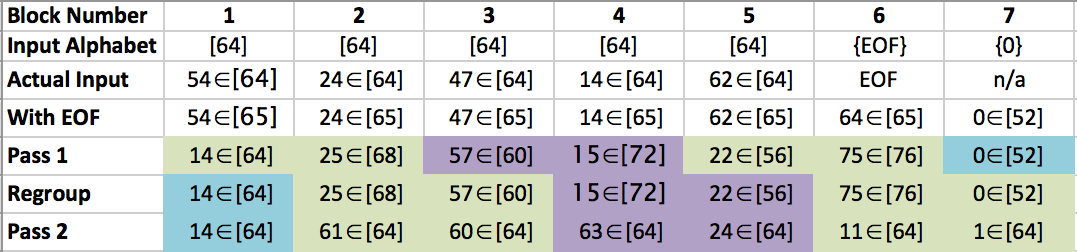
\includegraphics[scale=0.4]{problem1a-d}

{\bf Encoding of a:} \{14, 61, 60, 63, 24, 11, 1\} = \{e, Z, Y, " ", o, b, 1\}

Pass 1:

1st double block: encode (54, 24)$\in$ [65]x[65] as 2 numbers in range [64]x[68]

z = $24*65+54 = 1,614$

z \% 64 = $25*64+14$

1st double block = (14, 25) $\in$ [64]x[68]

2nd double block: encode (47, 14)$\in$ [65]x[65] as 2 numbers in range [60]x[72]

z = $14*65+47 = 957$

z \% 60 = $15*60+57$

2nd double block = (57, 15) $\in$ [60]x[72]

3rd double block: encode (62, 64)$\in$ [65]x[65] as 2 numbers in range [56]x[76]

z = $64*65+62 = 4,222$

z \% 56 = $75*56+22$

3rd double block = (22, 75) $\in$ [56]x[76]

Pass 2:

1st double block: encode (25, 57)$\in$ [68]x[60] as 2 numbers in range [64]x[64]

z = $57*68+25 = 3,901$

z \% 64 = $60*64+61$

1st double block = (61, 60) $\in$ [64]x[64]

2nd double block: encode (15, 22)$\in$ [72]x[56] as 2 numbers in range [64]x[64]

z = $22*72+15 = 1,599$

z \% 64 = $24*64+63$

2nd double block = (63, 24) $\in$ [64]x[64]

3rd double block: encode (75, 0)$\in$ [76]x[52] as 2 numbers in range [64]x[64]

z = $0*76+75 = 75$

z \% 64 = $1*64+11$

3rd double block = (11, 1) $\in$ [64]x[64]

{\bf Encoding of b:} \{29, 21, 62, 13, 27\} = \{t, l, ".", d, r\}

Recover Pass 2:

1st double block: encode (49, 7) $\in$ [64]x[64] as 2 numbers in range [68]x[60]

z = $7*64+49 = 497$

z \% 68 = $7*68+21$

1st double block = (21, 7) $\in$ [68]x[60]

2nd double block: encode (39, 48) $\in$ [64]x[64] as 2 numbers in range [72]x[56]

z = $48*64+39 = 3,111$

z \% 72 = $43*72+15$

2nd double block = (15, 43) $\in$ [72]x[56]

3rd double block: encode (10, 1) $\in$ [64]x[64] as 2 numbers in range [76]x[52]

z = $1*64+10 = 74$

z \% 76 = $0*76+74$

3rd double block = (74, 0) $\in$ [76]x[52]


Recover Pass 1:

1st double block: encode (50, 21) $\in$ [64]x[68] as 2 numbers in range [65]x[65]

z = $21*64+50 = 1,394$

z \% 65 = $21*65 + 29$

1st double block = (29, 21) $\in$ [65]x[65]

2nd double block: encode (7, 15) $\in$ [60]x[72] as 2 numbers in range [65]x[65]

z = $15*60+7 = 907$

z \% 65 = $13*65 + 62$

2nd double block = (62, 13) $\in$ [65]x[65]

3rd double block: encode (43, 74) $\in$ [56]x[76] as 2 numbers in range [65]x[65]

z = $74*56+43 = 4,187$

z \% 65 = $64*65+27$

3rd double block = (27, 64) $\in$ [65]x[65]

{\bf Encoding of c:} \{29, 21, 64\} = \{t, l\}

Recover Pass 2:

1st double block: encode (57, 9) $\in$ [64]x[64] as 2 numbers in range [68]x[60]

z = $9*64+57 = 633$

z \% 68 = $9*68+21$

1st double block = (21, 9) $\in$ [68]x[60]

Recover Pass 1:

1st double block: encode (50, 21) $\in$ [64]x[68] as 2 numbers in range [65]x[65]

z = $21*64+50 = 1,394$

z \% 65 = $21*65 + 29$

1st double block = (29, 21) $\in$ [65]x[65]

2nd double block: encode (9, 15) $\in$ [60]x[72] as 2 numbers in range [65]x[65]

z = $15*60+9 = 909$

z \% 65 = $13*65 + 64$

2nd double block = (64, 13) $\in$ [65]x[65]

\end{solution}
\fi

\end{itemize}




\newproblem{Zoo Dilemma}{10 points}

You own a zoo with $n$ animals. Some pairs of animals cannot co-exist
with each other (e.g., one will eat the other), while others can. You
worked hard, and developed a complete set of $m$ pairs of animals
which cannot co-exist. Design $O(m+n)$ algorithm to partition (if at
all possible) the animals into two groups, such that each animal in a
group can co-exist with every other animal in the same group.
\\ \hint{Use BFS on an appropriate graph and use the BFS tree to
derive the only {\em possible} partition. Then verify that this
partition is indeed OK.}

\ifnum\me<2
\begin{solution}

Input: Graph with animals as vertex, edges are between each vertex that {\bf cannot} coexist.

Algorithm:
Run BFS on any vertex, label root vertex as a part of group A.

During the BFS run, first consult the original graph to see if its edges between itself and another of the same group (i.e. A with an edge to A). If this is true, then it is not possible to divide the animals into just 2 groups, so break out of the algorithm.

Continuing in the BFS run, label the current vertex as a part of the opposite group as your predecessor (so if you came from a vertex in group A, label current vertex as in group B).

At the end of the BFS run, it will either be an unsolvable graph, or all the animals (vertices) in the graph are labeled as either in group A or B.

As the algorithm is basically a BFS run, our running time analysis is going to be:

T(n) = $\Theta$(m + n)
\end{solution}
\fi


\newproblem{Crazy Dogs}{15 points}

A fellow Moe and his buddy Joe live in a city $G=(V,E)$ which is an
undirected graph on $n$ verteces and $m$ edges, given in the adjacency
list form. Moe lives in a vertex $a$ and owns a crazy dog Mimi, while
Joe lives at a vertex $b$ and owns a crazy dog Kiki. This Sunday Moe
wants to take Mimi to a veterinarian clinic located at vertex $c$, while
Joe wants to take Kiki to the dance competition located at a vertex
$d$. One problem, though: the dogs hate each other, and if one of them
smells the other, all hell breaks lose. Luckily, they can smell each
other only if within distance at most $15$ in $G$, and you know that
$dist_G(a,b), dist_G(c,d)>15$. Moe and Joe would like to start at the
same time (with Moe and Mimi at $a$ and Joe and Kiki at $b$) and get
both dogs to their respective destinations $c$ and $d$ in the
smallest number of {\em steps} $t$. A {\em step} consists of both dogs
going to their respective neighboring verteces, or one dog going to a
neighboring vertex, and the other dog staying put, barking at the
pedestrians. Of course, such a step is possible only if the dogs stay
within distance $16$ or more both before and after the step.

Your job is to design an algorithm for Moe and Joe to compute $t$ (and
the optimal route), if the route exists, and analyze its running time.

\begin{itemize}

\item[(a)] Using one or more runs of the BFS algorithm on $G$, fill in the
matrix $OK[x,y]$, where $OK[x,y]=1$, if it is OK for Mimi to be at
vertex $x$ and Kiki to be at vertex $y$ at the same time, and $OK[x,y]=0$
otherwise. How long did it take you to fill this matrix $OK[x,y]$?

\ifnum\me<2
\begin{solution}

As matrix OK[x,y] is an (n x n) matrix, and we are going through the graph via BFS, which completes each row.

T(n) = rows * (BFS time)

T(n) = n * (m + n)

T(n) = n(m + n)
\end{solution}
\fi

\item[(b)]  Design a graph $H=(V',E')$ whose vertex set consists of
possible ``ok configurations'' for Mimi and Kiki, and whose edge set
represents the possible single steps of your algorithm. Be sure to
formally define $V'$ and $E'$ as functions of $V$ and $E$ and the matrix
$OK$ from part (a). How long (in the worst case) did it take you to create
an adjacency list for $H$ (not counting what you did in part (a))?
What is the maximum $|V'|$ and $|E'|$?

\ifnum\me<2
\begin{solution}

H = (V', E')

V' = \{$V_i V_j$ $|$ OK[i,j] == 1\}

E' = \{ ($v_i$, $v_j$) $|$ $v_i = v_{xy}$, $v_j = v_{yz}$
 \& $ OK[x, y] == 1$ \& $ OK[y, z] == 1$\}


Time to make adjacency list:

T(n) = 1 pass of BFS, so

$T(n) = \Theta(m + n)$

Maximum $|V'|$ = $|V^2| - |V|$

Maximum $|E'|$ = $\Theta(n^4)$
\end{solution}
\fi

\item[(c)] Describe the original problem as a shortest path computation
on $H$. Finally, solve the original problem, and help Moe and
Joe. Analyze the overall running time of your algorithm, as a function
of $n$ and $m$.

\ifnum\me<2
\begin{solution}

Run BFS on the start node:

BFS($v_{ab}$), and whatever is the shortest distance found at the end node $v_{cd}$ will be the shortest valid path for both Moe and Joe to reach their destinations.

T(n) = BFS

T(n) = $\Theta(m + n)$
\end{solution}
\fi

\end{itemize}


\end{document}
